\documentclass{standalone}

\usepackage{tikz}
\usetikzlibrary{intersections,decorations.markings}

\begin{document}
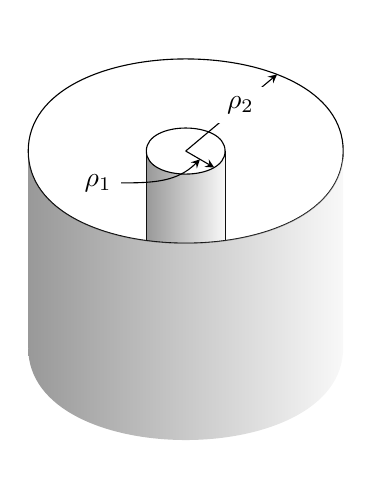
\begin{tikzpicture}
%\draw[thick,gray] (-3,-4) grid (3,3);
%\draw[thin,gray,step=0.2] (-3,-4) grid (3,3);

\begin{scope}
\clip (-2,0) to [out=-90,in=-90] (2,0)  to [out=90,in=90] (-2,0);
\draw(-2,0)--(-2,-2.5);
\draw(2,0)--(2,-2.5);

\draw(-0.5,0)--(-0.5,-1.5);
\draw(0.5,0)--(0.5,-1.5);

\shade[opacity=0.5,left color=black!80,right color=gray!10] (-0.5,0) to [out=-90,in=-90] (0.5,0) --++(0,-1.5) to [out=-90,in=-90] ++(-1,0)--cycle;
\end{scope}
%
\draw[name path=k1] (-2,0) to [out=-90,in=-90] (2,0)  to [out=90,in=90] (-2,0);
\draw[name path=k2] (-0.5,0) to [out=-90,in=-90] (0.5,0) to [out=90,in=90] (-0.5,0);
\shade[opacity=0.5,left color=black!80,right color=gray!10] (-2,0) to [out=-90,in=-90] (2,0) --++(0,-2.5) to [out=-90,in=-90] (-2,-2.5)--cycle;

\path[name path=k3] (0,0) --++(40:2);
\path[name path=k4] (0,0) --++(-30:1);

\draw[-stealth,name intersections={of=k1 and k3}](0,0)--(intersection-1)node[pos=0.6,fill=white]{$\rho_2$};
\draw[-stealth,name intersections={of=k2 and k4}](0,0)--(intersection-1)coordinate[pos=0.5](kk);
\draw[stealth-] (kk) to [out=-135,in=0] ++ (-1,-0.3)node[left]{$\rho_1$};




\end{tikzpicture}
\end{document} 
